\section{Evaluation}

\label{sec:experiments}

We evaluate the efficacy of the methods hitherto discussed by demonstrating that  
\begin{enumerate*}
    \item our fitness function is well-chosen i.e., that is correlates with performance measurements in real hardware; that
    \item our evolutionary process is capable of finding novel array layouts with favorable cache properties; and that
    \item the layouts which are found by our evolutionary process actually lead to relevant performance gains in real hardware.
\end{enumerate*}
Our validation is based on eight distinct access patterns and two processors with distinct cache hierarchies.

\subsection{Experimental Setup}

% \subsubsection{Access Patterns}
\begin{lstfloat}
\begin{lstlisting}[style=mystyle,frame=tlrb,basicstyle={\scriptsize\ttfamily},language=c++]
template <concepts::array<2> M>
void mm_ijk(const M & A, const M & B, M & C) {
    const auto m = C.get_size();
    for (std::size_t i = 0; i < m; ++i) {
        for (std::size_t j = 0; j < m; ++j) {
            typename M::value_type acc = 0.;
            for (std::size_t k = 0; k < m; ++k)
                acc += A.load(i, k) * B.load(k, j);
            C.store(acc, i, j);
        }
    }
}
\end{lstlisting}\vspace{-2mm}
\caption{Example of how an access pattern (\textsc{MMijk}) is described in C++. Metaprogramming allows the same source to be used for both simulation and execution on real hardware.}
\label{lst:mmijk_example}
\end{lstfloat}

We consider a set of eight access patterns loosely based on the selection of algorithms used by \citeauthor{10.1002/cpe.1018}~\cite{10.1002/cpe.1018}. The access patterns were picked to represent common real-world applications (dense linear algebra and fluid dynamics), to represent both two-dimensional and three-dimensional applications, and to differ in critical properties such as memory size and number of loads and stores. A description of the access patterns we consider in this paper is given in \cref{tab:pattern_stats}.

All our access patterns are described using C++ code---see the example in \cref{lst:mmijk_example}---which ensures high performance as opposed to the Python code used for our evolutionary processes; the interaction between the C++ and Python components of our project is managed using \textsc{pybind11}~\cite{pybind11}. We use template meta-programming to generalize our access patterns in such a way that a single definition can be used for both simulation and benchmarking without loss of performance due to run-time polymorphism; this eliminates any possible discrepancies between the code used for simulation and the code used for measurement.

\begin{table*}
    \centering
    \caption{Overview of the access patterns used for evaluation, including the use of memory and the number of loads and stores.}
    {\small
    \begin{tabular}{l p{8.7cm} r r r}
        \toprule
        Access pattern & Description & Mem.\ size & Loads & Stores  \\\midrule
        $\textsc{MMijk}(m; s)$ & Multiplication of two $2^m \times 2^m$ matrices, both of $s$-byte real numbers. & $3\cdot s \cdot 2^{2m}\,\si{\byte}$ & $2 \cdot 2^{3m}$ & $2^{2m}$ \\
        $\textsc{MMTijk}(m, n; s)$ & Multiplication of a $2^m \times 2^n$ matrix by a transposed $2^m \times 2^n$ matrix. & $s \cdot (2 \cdot 2^{m+n} + 2^{2n}) \si{\byte}$ & $2\cdot2^{2m+n}$ & $2^{2m}$ \\
        $\textsc{MMikj}(m; s)$ & Same as $\textsc{MMijk}(m;s)$ with the order of the inner loops switched. & $3\cdot s \cdot 2^{2m}\,\si{\byte}$ & $3 \cdot 2^{3m}$ & $2^{3m}$ \\
        $\textsc{MMTikj}(m, n; s)$ & Same as $\textsc{MMTijk}(m, n; s)$ with the order of the inner loops switched. & $s \cdot (2 \cdot 2^{m+n} + 2^{2n}) \si{\byte}$ & $3\cdot2^{2m+n}$ & $2^{2m+n}$ \\
        $\textsc{Jacobi2D}(m, n; s)$ & Four-point stencil kernel over a $2^m \times 2^n$ array of $s$-byte real numbers. & $2 \cdot s\cdot 2^{m+n}\,\si{\byte}$ & $\sim4 \cdot 2^{m + n}$ & $2^{m + n}$\\
        $\textsc{Cholesky}(m; s)$ & Cholesky--Banachiewicz decomposition of a $2^m \times 2^m$ matrix. & $2 \cdot s \cdot 2^{2m}\,\si{\byte}$ & $2 \cdot 2^{2m}$ & $\sim\frac{1}{2} \cdot 2^{2m}$\\
        $\textsc{Crout}(m; s)$ & Crout decomposition of a $2^m \times 2^m$ matrix of $s$-byte real numbers. & $2 \cdot s \cdot 2^{2m}\,\si{\byte}$ & $\frac{7}{2} \cdot 2^{2m}$ & $2^{2m}$ \\
        $\textsc{Himeno}(m, n, p; s)$ & Nineteen-point Himeno stencil \cite{himeno} over $2^m \times 2^n \times 2^p$ arrays. & $12\cdot s \cdot 2^{m + n + p}\,\si{\byte}$ & $24 \cdot 2^{m+n+p}$ & $2^{m+n+p}$\\
         \bottomrule
    \end{tabular}}
    \label{tab:pattern_stats}
\end{table*}

% \subsubsection{Hardware}

\label{sec:results:simulated_hardware}

\begin{lstfloat}
\begin{sublstfloat}[b]{0.49\columnwidth}
\begin{lstlisting}[style=mystyle,frame=tlrb,basicstyle={\scriptsize\ttfamily}]
caches:
  L1:
    sets: 64
    ways: 8
    line: 64
    replacement: LRU
    write_back: true
    store_to: L2
    load_from: L2
    latency: 4
  L2:
    sets: 512
    ways: 8
    line: 64
    replacement: LRU
    write_back: true
    store_to: L3
    load_from: L3
    victim_to: L3
    latency: 12
  L3:
    sets: 25600
    ways: 16
    line: 64
    replacement: LRU
    write_back: true
    latency: 36
memory:
  first: L1
  last: L3
  latency: 200
\end{lstlisting}\vspace{-2mm}
\caption{Intel Xeon E5-2660 v3}
\label{lst:cache_spec:haswell}
\end{sublstfloat}
\begin{sublstfloat}[b]{0.49\columnwidth}
\begin{lstlisting}[style=mystyle,frame=tlrb,basicstyle={\scriptsize\ttfamily}]
caches:
  L1:
    sets: 64
    ways: 8
    line: 64
    replacement: LRU
    write_back: true
    store_to: L2
    load_from: L2
    latency: 7
  L2:
    sets: 1024
    ways: 8
    line: 64
    replacement: LRU
    write_back: true
    store_to: L3
    load_from: L3
    victim_to: L3
    latency: 12
  L3:
    sets: 32768
    ways: 16
    line: 64
    replacement: LRU
    write_back: true
    latency: 46
memory:
  first: L1
  last: L3
  latency: 200
\end{lstlisting}\vspace{-2mm}
\caption{AMD EPYC 7413}
\label{lst:cache_spec:zen3}
\end{sublstfloat}
\caption{Two examples of cache specifications for different CPU models. Note that these configurations are approximations of the true cache hierarchies.}
\label{lst:cache_spec}
\end{lstfloat}

We conduct our experiments on two different CPUs: the Intel Xeon E5-2660~v3~\cite{e52660} based on the Haswell microarchitecture~\cite{6762795}, and the AMD~EPYC~7413~\cite{epyc7413} based on the Zen~3 microarchitecture~\cite{9718180}. When we perform experiments on non-simulated Haswell processors we use the \blind{the DAS-6 cluster~\cite{7469992}}, whereas we use \blind{a machine located at CERN} for experiments on Zen~3 processors. When we perform experiments based on simulation, we use the \blind{the DAS-6 cluster~\cite{7469992}} and configure our cache simulator according the cache configurations shown in \cref{lst:cache_spec:haswell} for the Haswell processor, and \cref{lst:cache_spec:zen3} for the Zen~3 processor. Note that the cache configurations are based on the accessibility of caches from a single core. This is especially relevant for the L3 cache on the Zen~3 chip, which is shared across groups of cores rather than the entire CPU: in the case of the AMD~EPYC~7413, the CPU comes equipped with \SI{128}{\mebi\byte} of L3 cache, but only \SI{32}{\mebi\byte} is accessible from any single core~\cite{9718180}. We simplify the cache replacement policies of the actual hardware by assuming LRU caches (i.e., caches with a least-recently-used eviction policy); in reality, the Haswell caches employ eviction policies consistent with tree-PLRU (tree-based pseudo-LRU) for the L1 and L2 caches~\cite{10.1145/3385412.3386008,10.1145/3297858.3304062}, while the L3 cache is consistent with a set-dueling-controlled adaptive insertion policy~\cite{4460516,10.1145/3297858.3304062}. Cache sizes were gathered from specification documents~\cite{amd19h,6762795}, while cache latencies were obtained optimistically from sources on the fastest load-to-use latencies~\cite{amd19h,hwbp}. The Zen~3 L1 cache has a fastest load-to-use latency of four cycles for integers and seven cycles for floating point values~\cite{amd19h}---we use the latter in our simulations. Finally, we assume a constant 200 cycle access latency for main memory in both systems.

\subsection{Fitness Function Validation}

\label{sec:res:fitval}

The fitness function we use in our evolutionary process (\cref{sec:exploration:fitness}) is based on simulation results because %Although we believe that 
simulation yields significant benefits over empirical measurements, primarily in terms of determinism and in the ability to simulate future hardware. However, this strategy is not without risk: the simulation we perform is based on a non-cycle-accurate simulator, uses simplified cache hierarchies, and ignores computation entirely. %Furthermore, and our cache hierarchies are approximations of the extremely complex cache designs that are used in modern hardware. 
Consequently, we must evaluate the usefulness of our fitness function by establishing its correlation with execution time in real hardware.

Ideally, the running time of a kernel using a given array layout would correlate inversely linearly with our fitness function, therefore ensuring two important properties. 
Firstly and most importantly, it guarantees that running time decreases monotonically with the value of the fitness function, such that an array layout with a higher fitness value is guaranteed to run more quickly; this allows us to establish a ranking of layouts and enables us to reliably select the best-performing array layout. 
Secondly, linear correlation guarantees proportionality between fitness and running time, which facilitates the weighted selection of individuals.

To evaluate the degree to which the aforementioned criteria are met, we randomly select one hundred array layouts for each of the eight access patterns given in \cref{tab:pattern_stats}. We then evaluate the simulated fitness and measure the running time in real hardware of each pair of array layout and access pattern. The fitness functions of the pairs are calculated in parallel, as they are designed to be deterministic and impervious to cache pollution or resource contention. The empirical benchmarks are performed sequentially, ensuring that the benchmark is the sole user of the processor caches. All measurements are repeated ten times, and we report the mean and standard deviation of the running time.

\begin{figure}
    \centering
    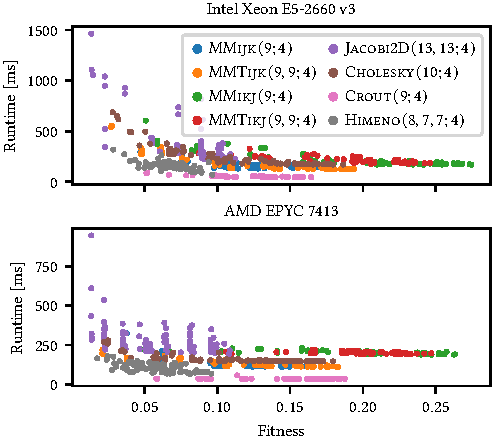
\includegraphics{figures/fitness_vs_runtime.pdf}
    \caption{Scatter plot of the fitness and measured running time on an Intel Xeon E5-2660 v3 CPU and AMD EPYC 7413 for randomly chosen array layouts.}
    \label{fig:fitness_corr}
\end{figure}

The results of this experiment are shown in \cref{fig:fitness_corr}. The coefficient of variation of the measurements never exceeded a value of $c_{\mathrm{v}} = 0.0801$. Accordingly, we have opted to omit error bars from the figure. Upon visual inspection, it is clear that the correlation between our fitness function and running time is not linear, although the two do appear correlated. We confirm our suspicions of correlation by computing Pearson's coefficient of correlation ($\rho_p$) and Spearman's coefficient of rank correlation ($\rho_s$); the resulting statistics are given in \cref{tab:correlation_table}. We observe that our fitness function and running time correlate moderately to strongly with running time for the Intel Xeon E5-2660 v3 processor, although the correlation is weaker for the AMD EPYC 7413 processor. Although it is clear that there is space for the fitness function to be improved, we believe that it correlates sufficiently with running time to enable its use in genetic algorithms.

\begin{table}
    \centering
    \caption{Pearson's coefficient of correlation ($\rho_p$) and Spearman's coefficient of rank correlation ($\rho_s$) between our simulation-based fitness function and true running time.}
    \begin{tabular}{l R{1cm} R{1cm} R{1cm} R{1cm}}
        \toprule
        & \multicolumn{2}{c}{Intel E5-2660 v3} & \multicolumn{2}{c}{AMD EPYC 7413} \\\cmidrule(lr){2-3}\cmidrule(lr){4-5}
        Access pattern & $\rho_{p}$ & $\rho_{s}$ & $\rho_{p}$ & $\rho_{s}$ \\\midrule
        $\textsc{MMijk}(9; 4)$ & \num{-0.672} & \num{-0.480} & \num{-0.648} & \num{-0.489} \\
        $\textsc{MMTijk}(9, 9; 4)$ & \num{-0.810} & \num{-0.896} & \num{-0.863} & \num{-0.823} \\
        $\textsc{MMikj}(9; 4)$ & \num{-0.845} & \num{-0.815} & \num{-0.800} & \num{-0.838} \\
        $\textsc{MMTikj}(9, 9; 4)$ & \num{-0.777} & \num{-0.744} & \num{-0.291} & \num{-0.405} \\
        $\textsc{Jacobi2D}(13, 13; 4)$\hspace{-2mm} & \num{-0.760} & \num{-0.769} & \num{-0.390} & \num{-0.428} \\
        $\textsc{Cholesky}(10; 4)$ & \num{-0.827} & \num{-0.953} & \num{-0.725} & \num{-0.892} \\
        $\textsc{Crout}(9; 4)$ & \num{-0.846} & \num{-0.663} & \num{-0.213} & \num{-0.704} \\
        $\textsc{Himeno}(8, 7, 7; 4)$ & \num{-0.607} & \num{-0.475} & \num{-0.561} & \num{-0.496} \\
        \bottomrule
    \end{tabular}
    \label{tab:correlation_table}
\end{table}

\subsection{Genetic Algorithm Performance}

\label{sec:expr:evolution}
%Having evaluated the validity of our fitness function, we proceed 
To evaluate our evolutionary process (\cref{sec:exploration}) as a whole,  
%In these experiments, 
we intend to verify that it can, indeed, find Morton-like array layouts that have a higher simulated fitness than the canonical layouts. To this end, we perform the evolutionary process for each combination of our two simulated processors and eight access patterns, giving rise to a total of sixteen experiments. For all of these experiments, we configure our genetic algorithm to use $\mu = 20$, $\lambda = 20$, and a mutation rate of $25\%$. We simulate a total of \num{20} generations in each case.

\cref{fig:fitness_violin} shows a violin plot of the fitness distribution of all individuals considered during the evolutionary process. \cref{fig:fitness_evolution} shows the evolution of population fitness over the course of our experiments. Note that each of these experiments represents a single evolutionary process. We notice that for the \textsc{MMTijk}, \textsc{MMikj}, \textsc{Jacobi2D}, and \textsc{Himeno} access patterns, our method does not manage to discover any layouts with higher fitness than the initial population of canonical layouts. In the experiment on the \textsc{MMijk} access pattern, we discover layouts with a fitness $149.8\%$ higher than the canonical layouts on the Intel Xeon E5-2660 v3 processor, and we improve on the fitness of canonical layouts by $187.5\%$ for the AMD EPYC 7413. We also find layouts with improved fitness for the \textsc{MMTikj} ($109.6\%$ and $141.1\%$ for the Intel and AMD processors, respectively), \textsc{Cholesky} ($26.4\%$ and $36.8\%$), and \textsc{Crout} ($545.9\%$ and $541.1\%$) access patterns. It is notable that we are able to find layouts with high fitness in few generations.

\begin{figure}
    \centering
    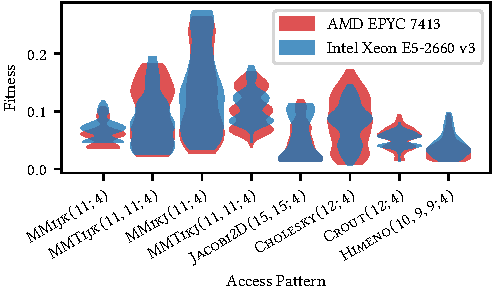
\includegraphics{figures/fitness_violin.pdf}
    \caption{Distribution of the fitness values for all individuals found across evolution experiments for eight access patterns and two processors.}
    \label{fig:fitness_violin}
\end{figure}

\begin{figure}
    \centering
    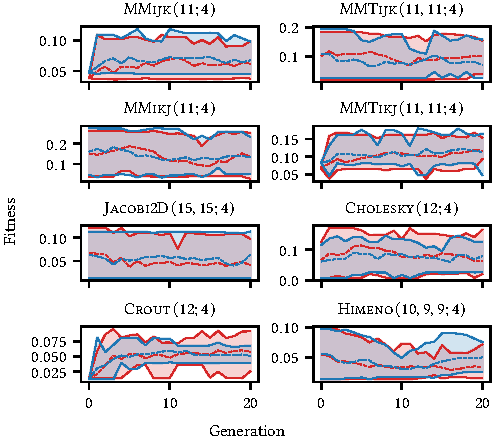
\includegraphics{figures/fitness_evolution.pdf}
    \caption{Range of fitness values across eight experiments for the Intel Xeon E5-2660 v3 (blue) and AMD EPYC 7413 (red). Mean fitness values are given by the dashed lines.}
    \label{fig:fitness_evolution}
\end{figure}

\subsection{Real-World Performance}

\label{sec:results:real-world}

In order to evaluate whether the layouts identified by our evolutionary algorithms as superior to canonical layouts are indeed better, we evaluate them on real hardware. We collect the fittest individual from each of the successful evolution experiments---i.e., experiments in which our method improved upon canonical layouts, as indicated by the top boundary in \cref{fig:fitness_evolution} exceeding the maximum fitness in the first generation---and evaluate the performance of those layouts compared to the canonical layouts on real hardware. Given that our genetic algorithm discovered superior layouts for four access patters---\textsc{MMijk}, \textsc{MMTikj}, \textsc{Cholesky}, and \textsc{Crout}--and that we evaluate a discovered layout and two canonical layouts for each access pattern, this gives rise to twenty-four experiments. We repeat each experiment ten times to compensate for run-to-run variance.

The results of our experiments are shown in \cref{tab:speedup_table}; they show that some access patterns---the \textsc{Cholesky} pattern in particular---benefit very little from our method, with speed-ups ranging from small on the Haswell processor to insignificant on the Zen 3 processor. The matrix multiplication access patterns benefit more, and performance for these access patterns is improved significantly. The \textsc{Crout} access pattern stands out as achieving very large speedup---up to a factor ten---from our method. It is worth noting that, in most cases, the Zen 3 processor benefits more from our evolutionary methodology than the Haswell processor; we do not currently have a satisfactory explanation for this behavior.

\begin{table}
    \centering
    \caption{Comparison of running time between the best-performing canonical layout and the best-performing layout found by our evolutionary process for four access patterns.}
    \begin{tabular}{l l S[table-format=3.2,table-space-text-post = \,\si{\second}] S[table-format=3.2,table-space-text-post = \,\si{\second}] r}
    \toprule
    \multicolumn{2}{l}{Access pattern} & {Best can.} & {Best evo.} & {Speedup} \\\midrule
    \multicolumn{2}{l}{Intel Xeon E5-2660 v3} & \\
    & $\textsc{MMijk}(11; 4)$ & 17.84\,\si{\second} & 10.94\,\si{\second} & $63.1\%$ \\
    & $\textsc{MMTikj}(11, 11; 4)$ & 18.13\,\si{\second} & 13.96\,\si{\second} & $29.9\%$ \\
    & $\textsc{Cholesky}(12; 4)$ & 11.84\,\si{\second} & 11.43\,\si{\second} & $3.6\%$ \\
    & $\textsc{Crout}(12; 4)$ & 158.54\,\si{\second} & 43.72\,\si{\second} & $262.6\%$ \\
    \multicolumn{2}{l}{AMD EPYC 7413} & \\
    & $\textsc{MMijk}(11; 4)$ & 37.71\,\si{\second} & 9.58\,\si{\second} & $293.8\%$ \\
    & $\textsc{MMTikj}(11, 11; 4)$ & 32.35\,\si{\second} & 15.21\,\si{\second} & $112.6\%$ \\
    & $\textsc{Cholesky}(12; 4)$ & 9.72\,\si{\second} & 9.55\,\si{\second} & $1.0\%$ \\
    & $\textsc{Crout}(12; 4)$ & 232.84\,\si{\second} & 21.03\,\si{\second} & $1007.0\%$ \\
    \bottomrule
    \end{tabular}
    \label{tab:speedup_table}
\end{table}

It is important to note that we do not claim to have discovered a novel way of performing matrix multiplication or matrix decomposition that outperforms existing implementations. Indeed, our experiments are based on relatively naive implementations of these algorithms; high-performance implementations of matrix multiplication commonly rely on tiling to significantly improve the cache behavior of the application~\cite{1214317}, and the performance of tiled matrix multiplication surpasses what we achieve in this paper. The purpose of the methodology described in this paper, rather, is to provide an alternative way of improving the cache behavior of an application in a manner which is fully agnostic of the application: unlike tiling and other application-specific optimizations, our methodology of altering the array layouts can be applied to any multi-dimensional problem without the need for application-specific knowledge. In addition, our approach requires few code changes, making it easy to implement.